%%%% Proceedings format for most of ACM conferences (with the exceptions listed below) and all ICPS volumes.
\documentclass[sigconf]{acmart}
%%%% As of March 2017, [siggraph] is no longer used. Please use sigconf (above) for SIGGRAPH conferences.

%%%% Proceedings format for SIGPLAN conferences 
% \documentclass[sigplan, anonymous, review]{acmart}

%%%% Proceedings format for SIGCHI conferences
% \documentclass[sigchi, review]{acmart}

%%%% To use the SIGCHI extended abstract template, please visit
% https://www.overleaf.com/read/zzzfqvkmrfzn

\usepackage{booktabs} % For formal tables
\usepackage[ruled]{algorithm2e}
\renewcommand{\algorithmcfname}{ALGORITHM}
\SetAlFnt{\small}
\SetAlCapFnt{\small}
\SetAlCapNameFnt{\small}
\SetAlCapHSkip{0pt}
\IncMargin{-\parindent}
\SetKw{Initialize}{initialize}
\SetKw{Trace}{traceback}
\SetKw{Set}{set}
\SetKw{Return}{return}




% Copyright
%\setcopyright{none}
%\setcopyright{acmcopyright}
%\setcopyright{acmlicensed}
\setcopyright{rightsretained}
%\setcopyright{usgov}
%\setcopyright{usgovmixed}
%\setcopyright{cagov}
%\setcopyright{cagovmixed}


% DOI
\acmDOI{}

% ISBN
\acmISBN{}

%Conference
\acmConference[]{}{}{} 
\acmYear{}
\copyrightyear{2017}

\acmPrice{0.00}


\begin{document}
\title{Text Re-use and Paraphrase Detection with Semantical Smith-Waterman Local Alignment}
\subtitle{Extended Abstract}
%\subtitlenote{The full version of the author's guide is available as
 % \texttt{acmart.pdf} document}


\author{Alexander C. Furnas}
\affiliation{%
  \institution{Department of Political Science, University of Michigan}
}
\email{zfurnas@umich.edu}


% The default list of authors is too long for headers}
\renewcommand{\shortauthors}{AC Furnas}


\begin{abstract}
This paper details a new method for detecting text reuse and paraphrasing. The method proposed is an extension of the Smith-Waterman local alignment algorithm with semantically aware mismatch penalties. This modification enables detection of instances of text reuse in which words are changed to semantically similar alternatives to fit new contexts or disguise the source of the text.  
\end{abstract}

%
% The code below should be generated by the tool at
% http://dl.acm.org/ccs.cfm
% Please copy and paste the code instead of the example below. 
%
% We no longer use \terms command
%\terms{Theory}

\keywords{Text Reuse, Information Retrieval, Natural Language Processing, Smith-Waterman, Semantic Similarity, Local Alignment}

%% Used in some conference proceedings e.g. sigplan and sigchi
% \begin{teaserfigure}
%   \includegraphics[width=\textwidth]{sampleteaser}
%   \caption{This is a teaser}
%   \label{fig:teaser}
% \end{teaserfigure}

\maketitle

\section{Problem}
A substantial sub-literature in political science has focused on patterns of collaboration and coordination among members of Congress. Indeed we may think of different types of collaboration. \cite{fenno1978home} argues that members are motivated by three primary goals: re-election, power within the institution, and good public policy. To achieve these goals they may collaborate or coordinate with other members.

Cosposorship as collaboration

Dear collegue collaboration

semantic burst collaboration



Co-sponsoring legislation may be the most studied form of between member collaboration \citep{zhang2008community,fowler2006connecting, koger2003position}  . \cite{zhang2008community} use network theory to explore the community structure of cos-sponsorship, and observe polarization.  
At the state level \cite{bratton2011networks



 of the kind demonstrated by TKTK can be seen as intra-institutional collaboration that serves ultimate policy goals, as well as currying favor among their colleagues to increase their standing within the institution. Fundraising through leadership PACs 


At t



In recent years, scholars in political science have begun using natural language processing techniques to analyze vast troves of politically relevant text \cite{grimmer2013text}. This work has applied techniques ranging from topic modeling \cite{roberts2014structural} to scaling to recover latent traits \cite{lowe2013validating}. A recent body of work has begun to detect text reuse in political texts, particularly for modeling diffusion \cite{smith2013infectious,smith2014detecting}. This work has adapted the Smith-Waterman local alignment algorithm (SW, hereafter) \cite{smith1981identification}, which was originally developed in biostatistics to find the optimal local alignments of sequences of nucleic acids, for text purposes.

Wilkerson and colleagues have used SW to find previous bills which contained portions of what eventually became the Affordable Care Act. This same method has been used to identify state bills that share text, to determine instances of policy diffusion \cite{Fridolin2017text} or find sufficiently similar state bills to use as bridging observations in a pooled IRT estimation of state legislator ideology \cite{Furnas2017ideal}.   

SW is an effective algorithm for finding examples of exact text reuse, or reuse of exact text with additional text insertions. A global text alignment algorithm, like the Needleman-Wunsch, would do a poor job of detecting text from string $A$ reused in string $B$, if $B$ were identical to $A$ but with a new appositional phrase inserted in the middle\cite{needleman1970general}. 

SW is a dynamic programming algorithm that computes all of the possible alignments of two sequences, tabulating scores according to a bonus for aligned items, a penalty for mismatching items and a penalty for the insertion of gaps. Backpointers to previous parts of the alignment are stored in a table. The maximum possible score is found, and then backpointers are used to determine what path of the possible alignments yielded that optimal alignment. In this way it is similar to an edit distance calculation. All misalignments, that is cases where words in the two sequences do not match, are treated the same.

To date, SW has been by political scientists used largely to detect the reuse of legislative text. In a legislative context, where changing a single ``shall" to a ``may" can significantly alter the meaning of a provision, exact matches may be the appropriate form of text reuse to detect. However, in other forms of political text or speech we may be interested in a more flexible form of text reuse. SW is less effective for detecting instances of reuse in which moderate paraphrasing or adaptation has been done. This is especially relevant in the context of political speech, as two actors offering essentially the same message may need to adapt it to fit their circumstances. 

I propose a modification of the standard SW algorithm in to better detect this adaptive reuse. This modified version is called the Semantic Smith-Waterman (SSW. hereafter). Rather than treating all mismatches the same, the method proposed here scores each mismatch according to word similarity in a semantic space and weights these mismatches accordingly. The more similar the two words are the less the mismatch is penalized.  

\section{Method}


Consider a hypothetical legislator expressing  one of the following sentiments:

\textbf{A:} \emph{"My esteemed colleague is resident of the state of Michigan, and clearly proud of it."}
 
\textbf{B:} \emph{"My esteemed colleague is resident of the state of denial, and clearly proud of it."}
 
In statement A, the legislator is making a straightforward statement about the state of residence of their colleague. In statement B, the legislator is making an ironic statement about their colleague's inability to confront facts. While the text in these two instances is almost exactly the same, their meanings are notably different. 

Now consider a second hypothetical legislator, making the following statement: 

\textbf{C:} \emph{"My esteemed colleague is resident of the state of Ohio, and clearly proud of it."}

Is statement C more similar to A or B? The standard SW algorithm would say that C is equally as similar to A as it is to B. C aligns with A and B perfectly except for one mismatch (``Michigan" --- ``Ohio" and ``denial" --- ``Ohio") which are penalized equally according to a constant.

The SSW scores these differently. The mismatch penalty applied depends on the relationships between the words in a semantic space. 

In the application of SSW presented here, words are compared in a google's pre-trained 300 dimension \texttt{word2vec} word embeddings. 

Algorithm \ref{alg:one} provides a detailed explication of the the SSW algorithm. The algorithm functions nearly identically to the standard SW, except that mismatches are scored according to a similarity function rather than penalized with a constant. The similarity score $s(a,b)$ for two words $a$ and $b$ is derived according to the scoring function described in Algorithm \ref{alg:semsim}.

The SSW consists of the same four steps as SW: 1) Choice of scoring parameters, 2) the scoring and traceback matrices are initialized, 3) the scoring matrix is filled, and backpointers stored in the traceback matrix, 4) traceback starting from the highest scoring cell in the scoring matrix.



% Algorithm
\begin{algorithm}[t]
\SetAlgoNoLine
\KwIn{Two sequences of words, $A$ and $B$, such that $A=a_{1}a_{2}... a_{n}$ and $B=b_{1}b_{2}... b_{m}$ where $n$ and $m$ are the lengths of $A$ and $B$ respectively.}
\KwOut{Optimal semantically aware local alignment of A and B with gaps, alignment score}
\Initialize{Scoring matrix $\mathbf{H}$}{ with dimensions $(n+1) \times (m+1)$, \\ \hspace{33pt}$ H_{k0}=H_{0l}=0\quad for\quad 0\leq k\leq n\quad and\quad 0\leq l\leq m$;} 

\Initialize{Traceback matrix $\mathbf{T}$}{ with dimensions $(n) \times (m)$;}

 \For{each node $i$ in $j$ in $1:n+1, 1:m+1$}{
 
${\displaystyle H_{ij}=\max {\begin{cases}H_{i-1,j-1}+s(a_{i},b_{j}),\\H_{i-1,j}-W,\\H_{i,j-1}-W,\\0\end{cases}}}$
 
\vspace{10pt} 
\textbf{where}

$H_{i-1,j-1}+s(a_{i},b_{j})$ is the semantically weighted score of aligning $a_{i}$ and $b_{j}$,

$H_{i-1,j}-W_{1}$ is the score if $a_{i}$ is at the end of a gap,

$H_{i,j-1}-W_{1}$ is the score if $b_{j}$ is at the end of a gap,


\vspace{10pt}

 ${\displaystyle T_{ij}={\begin{cases}    (i-1,j-1), & \text{if } H_{ij} = H_{i-1,j-1}+s(a_{i},b_{j}) \\
    (i-1,j), & \text{if } H_{ij} = H_{i-k,j}-W \\
    (i,j-1), & \text{if } H_{ij} = H_{i,j-l}-W
    \end{cases}}}$
}

\Trace{Starting at $H_{ij}$ = $max(\mathbf{H})$}{\\
alignment = []

\While{$H_{ij} > 0$}{
append $T_{ij}$ to alignment

\Set{$i$,$j$}{ to $T_{ij}$}}
 
}

\Return{score = $max(\mathbf{H})$, alignment = alignment}

\caption{Semantic Smith Waterman\protect\footnotemark}
\label{alg:one}
\end{algorithm}

\subsection{Semantic mismatch scoring}
At this point it some additional explanation of the semantic mismatch scoring used here is warranted at is the principal difference between SW and SSW. Standard SW generally imposes a constant penalty for a mismatch, and then either a linear penalty for gap scoring or an affine gap penalty (where there is a greater penalty for creating than extending a gap). For simplicity's sake implementation described here uses only the simple linear gap penalty although there is no reason that SSW could not be extended to include affine gap scoring as well.

This implementation makes a few other simplifying assumptions that could be parameterized in a future implementation of SSW. These are as follows:

\begin{itemize}
\item Cosine similarity of \texttt{word2vec} word vectors is used as the similarity measure.
\item Cosine similarity scores below .5 are considered a mismatch and standard constant mismatch penalty is applied.
\item The constant mismatch penalty is set to be the same as the constant gap penalty $W$.
\item Perfect matches are set given a positive score twice the magnitude of the gap/mismatch penalty.\footnote{this matches the most common or default ratio between gap and match penalties uses in most applications of the standard SW.}
\item
\end{itemize}
  
Algorithm \ref{alg:semsim} shows this implementation. Here, $\mathbf{V}$ is a vector space from the \texttt{word2vec} word embeddings. 

\begin{algorithm}[t]
\SetAlgoNoLine
\KwIn{Two words, $a$ and $b$.}
\KwOut{An alignment score, $s(a,b)$ to be used in the Semantic Smith-Waterman alignment}
\If{$a=b$}{score $= 2W$}
\ElseIf{$a$ is a stop word or $b$ is a stop word}{score $= -W$}
\Else{$s= \cos(\mathbf{V}[a], \mathbf{V}[b]) -.5$

score$ =  2W s$ }
\caption{Semantically Weighted Alignment Score}
\label{alg:semsim}
\end{algorithm}


\subsection{Initialization}
The scoring matrix is initialized to with the words from string $A$ along the rows and from string $B$ along the columns, but with a first row and column set to 0. The result is a matrix with dimensions $(n+1)\times (m+1)$. Here, $n$ is the number of words in $A$ and $m$ is the number of words in $B$.

The traceback matrix is initialized to be size $n \times m$. 

\subsection{Scoring}
As cells in the scoring matrix are filled,as shown in Figure \ref{fig:score}, a pointer is stored in the traceback matrix indicating which of the neighboring cells provided the max value for $H_{i,j}$.

\begin{figure}
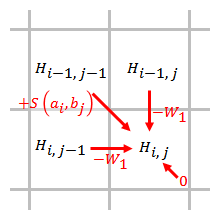
\includegraphics[width=.8\columnwidth]{Smith-Waterman-Algorithm-Scoring-1.png}
\caption{Scoring and Traceback. Source: Wikimedia Commons}
\label{fig:score}
\end{figure}

\footnotetext{Notation and explication for the Semantic Smith-Waterman used here is adapted from the Wikipedia article for the standard Smith-Waterman.} 

\subsection{Traceback}
The cell in the traceback matrix that corresponds to the cell in the scoring matrix which provides the maximum value is used as the starting position for traceback. Starting from this cell, the backpointers are used to determine the optimal local alignment of the two strings. Backtracing ends when the corresponding cell in the scoring matrix reaches 0.

\section{Empirical application}
Initially the plan was to use the PAN-15 plaigarism detection corpus to validate this new approach\cite{potthast2010evaluation}. However, after further investigating this evaluation it was found to be inappropriate. The PAN approach treats plagiarism as a classification problem, which supervised machine learning models are trained on a pre-classified corpus of instances of plagiarism and then out of sample predictions are made on a test corpus. SSW is a method not for categorical classification, but rather identification of local subsequences with scalar similarity scores. Evaluating SSW according using the PAN corpora would introduce additional score cut-point parameter, to determine whether a given local alignment was significant enough to indicate a classification of plagiarism. This is not the problem that SSW is created to solve, and as such the planned evaluation approach was abandoned. It is likely that the PAN corpora may still be useful for future evaluation and validation, but more work would be needed to determine how to adapt this data.

Instead, I decided to find an interesting empirical application and compare the performance of SW and SSW qualitatively. To explore the utility of this new approach to text reuse detection, I applied both SW and SSW to a corpus of tweets of Members of Congress and congressional candidates during the 2016 election cycle.\footnote{These tweets were kindly shared with me by Joseph DiGrazia, and when he publishes something with this corpus, any work that I produce validating this measure using this corpus will cite him.}

This corpus contains $893168$ non-retweet tweets from $714$ different accounts. Of these I took the first $100000$ tweets and looked for optimal local alignments in the rest of the $893168$ tweet corpus with both SW and SSW. These algorithms are computationally expensive, as they are $O(nm)$. Checking for each optimal alignment would require this be done $100000 \times 893168 \approx 8.93 \times 10^{10}$ times. To shrink the search space, I compared all documents to each other in a simple vector space constructed using \texttt{nltk} and \texttt{gensim}. Because I wanted to find results with as similar exact words as possible to each other, I did no transformations on this vector space, and did not remove stop words. Each tweet was then compared to the 100 closest tweets in this vector space using both SW and SSW. The scaling parameter/ gap penalty W was set to 10 for these trials.

Below I present the distributions of these similarity scores. Note, of course, that the sample of similarity scores calculated is a non-random sample of similarities between these tweets because of how the search space was constrained. 

\begin{figure}
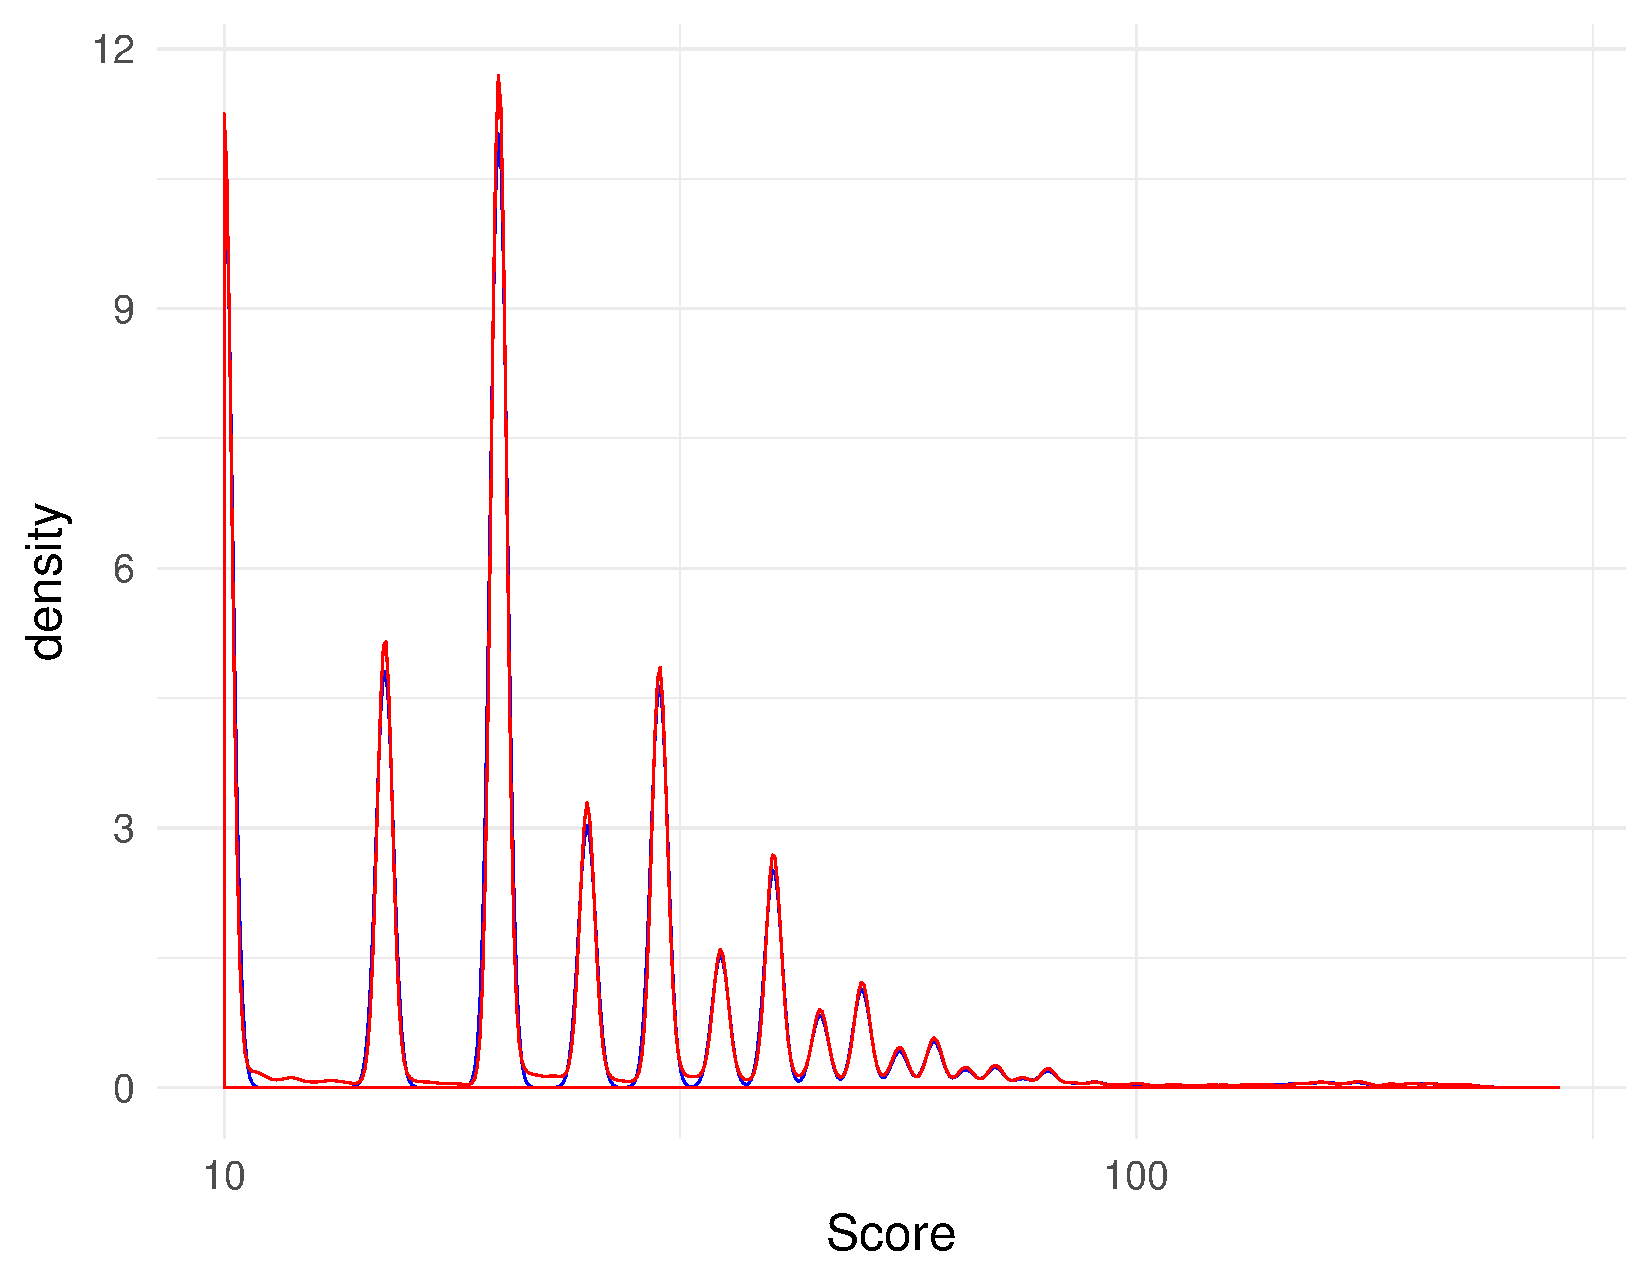
\includegraphics[width=.8\columnwidth]{Score_densities.pdf}
\caption{Smith-Waterman and Semantic Smith-Waterman Score densities}
\label{fig:scoredist}
\end{figure}

As Figure \ref{fig:scoredist} shows, these scores are highly similar, of course, but the interesting results come in the instances where SSW is substantially different from SW. 

SSW yields strictly higher scores than SW, as the semantic similarity score defaults to the standard mismatch penalty if the semantic similarity score is negative. The distribution of these differences is shown in Figure \ref{fig:scorediff} for all cases where that difference is non-zero.



\begin{figure}
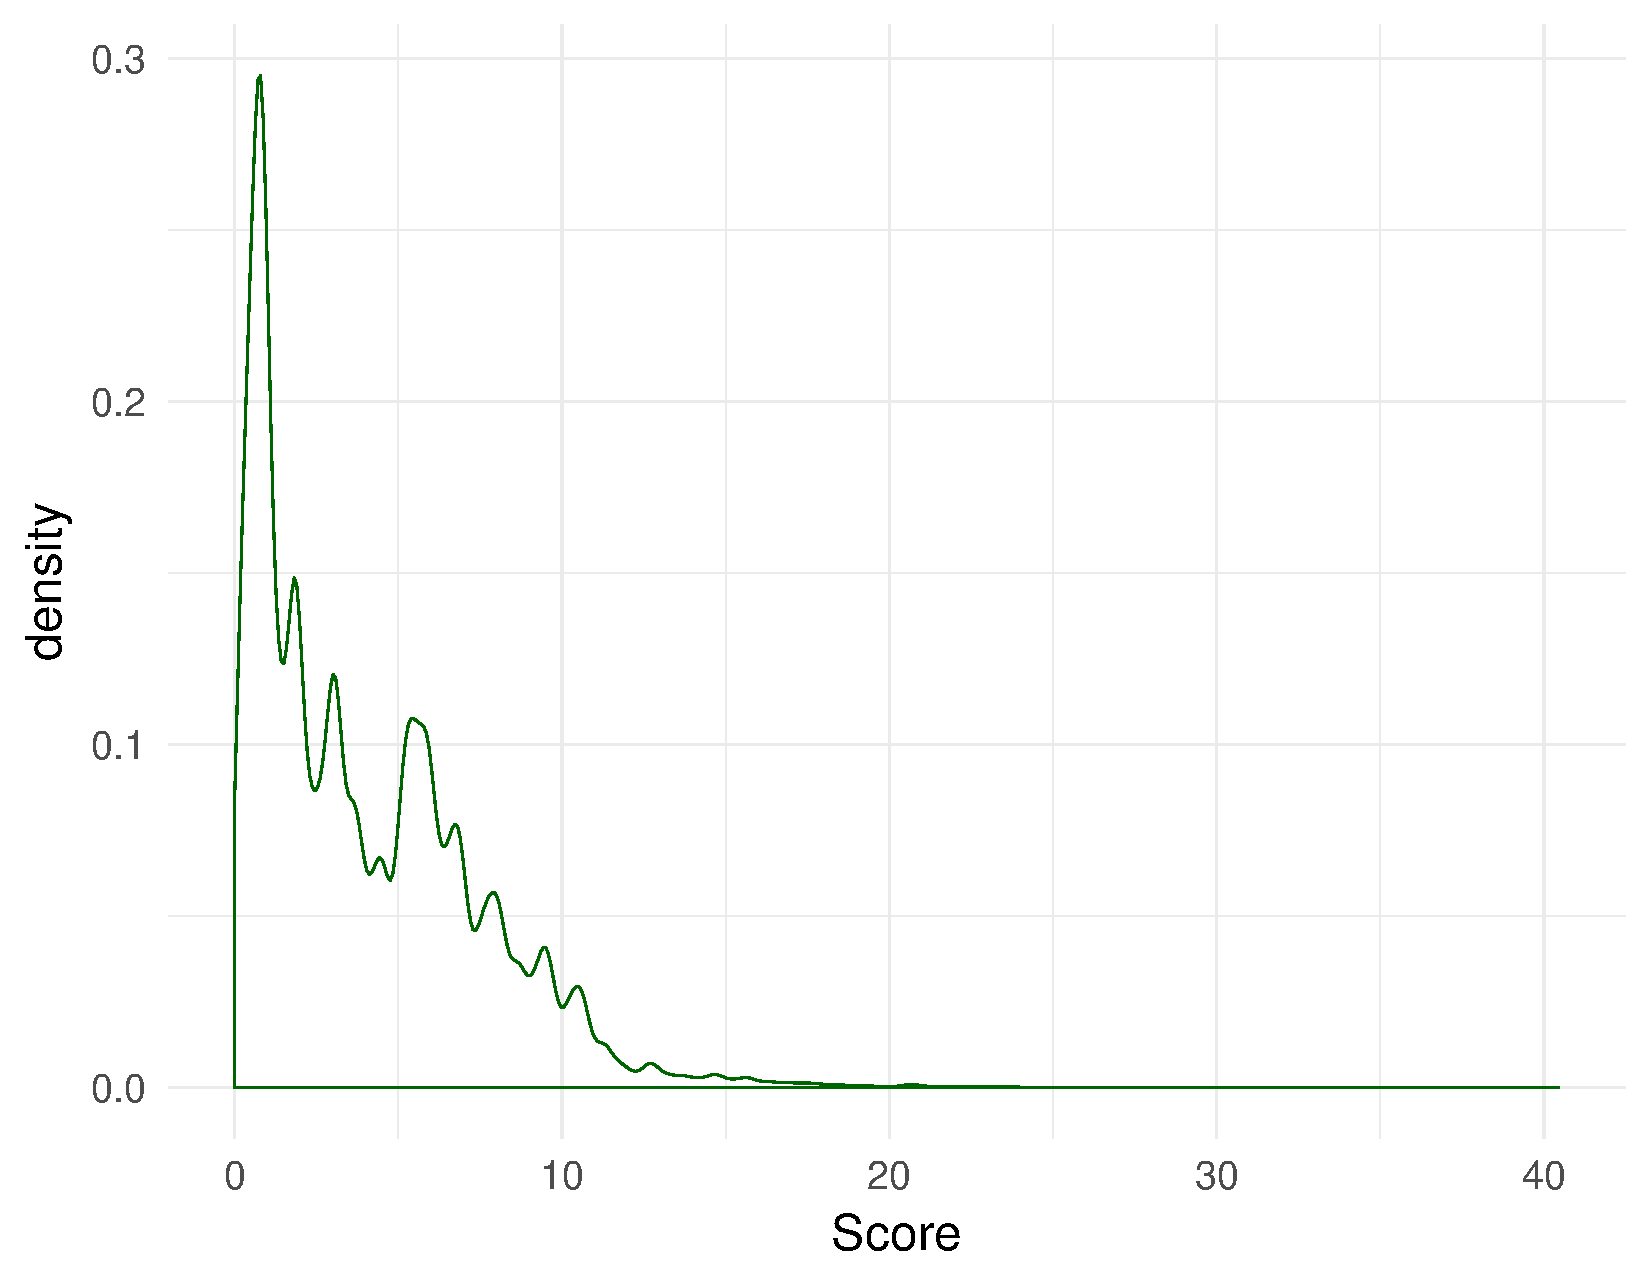
\includegraphics[width=.8\columnwidth]{Score_Diff.pdf}
\caption{Density of difference between Smith-Waterman and Semantic Smith-Waterman Score densities}
\label{fig:scorediff}
\end{figure}

See the Table \ref{tbl:diff} for the top most different matches.

% Please add the following required packages to your document preamble:
% \usepackage[normalem]{ulem}
% \useunder{\uline}{\ul}{}
\begin{table}[]
\tiny
\centering
\caption{Tweet pairs with the largest difference between SW and SSW}
\label{tbl:diff}
\begin{tabular}{|p{.1\columnwidth}|p{.1\columnwidth}|p{.4\columnwidth}|p{.4\columnwidth}|}
\hline
sw score & ssw score                   & query doc                                                                                                                                               & result doc                                                                                                                                          \\ \hline
50       & 90.453                      & Happy Memorial Day!! Thank you to all the brave women and men who've served our country to keep us free!                                                & Thank you to all brave men and women serving our nation and keeping us safe. \#ArmedForcesDay https://t.co/xVswnTWMR0                               \\ \hline
40       & 79.346 &Good luck to the @CSHighSchool girls soccer team as they play in the state semifinals. Go Lady Cougars! http://t.co/Zf4MTANhNM     & Good luck to the Thorndale Boys Basketball Team in their semifinal game of the 2A State Tournament. Go Bulldogs! https://t.co/tEMMW7QsCD            \\ \hline
45       & 82.277                      & As \#BlackHistoryMonth comes to a close, let us always celebrate the many contributions African Americans have made to improve our nation.              & As \#HispanicHeritageMonth draws to a close join me in celebrating the many contributions Latinos make to our nation. https://t.co/kpeMo6UlKI       \\ \hline
90       & 126.524                     & My heart goes out to those impacted by these heinous attacks in \#Paris. Please keep the victims and their families in your prayers.                    & My heart goes out to everyone affected by the horrific shooting in Orlando. I am keeping the victims and their families in my prayers.              \\ \hline
45       & 81.128                      & Good luck to the La Vega Girls Basketball Team as they play for the 4A State Championship. Go Lady Pirates! https://t.co/M4zQJTO0j6                     & Good luck to the Thorndale Boys Basketball Team in their semifinal game of the 2A State Tournament. Go Bulldogs! https://t.co/tEMMW7QsCD            \\ \hline
45       & 81.128                      & Good luck to the Thorndale Boys Basketball Team in their semifinal game of the 2A State Tournament. Go Bulldogs! https://t.co/tEMMW7QsCD                & Good luck to the La Vega Girls Basketball Team as they play for the 4A State Championship. Go Lady Pirates! https://t.co/M4zQJTO0j6                 \\ \hline
55       & 90.810                      & Many thanks to everyone who participated in the second annual Napa Valley Walk to End Alzheimer's. http://t.co/wHa18ZeWHf                               & Many thanks to all those who are participating in this morningŐs third annual Napa Valley Alzheimer's walk. http://t.co/DBcU95Ljbl                  \\ \hline
55       & 90.810                      & Many thanks to everyone who participated in the second annual Napa Valley Walk to End Alzheimer's. http://t.co/wHa18ZeWHf                               & Many thanks to all those who are participating in this morningŐs third annual Napa Valley Alzheimer's walk. http://t.co/DBcU95Ljbl                  \\ \hline
55       & 90.810                      & Many thanks to everyone who participated in the second annual Napa Valley Walk to End Alzheimer's. http://t.co/wHa18ZeWHf                               & Many thanks to all those who are participating in this morningŐs third annual Napa Valley Alzheimer's walk. http://t.co/DBcU95Ljbl                  \\ \hline
55       & 90.810                      & Many thanks to everyone who participated in the second annual Napa Valley Walk to End Alzheimer's. http://t.co/wHa18ZeWHf                               & Many thanks to all those who are participating in this morningŐs third annual Napa Valley Alzheimer's walk. http://t.co/DBcU95Ljbl                  \\ \hline
55       & 90.810                      & Many thanks to all those who are participating in this morningŐs third annual Napa Valley Alzheimer's walk. http://t.co/DBcU95Ljbl                      & Many thanks to everyone who participated in the second annual Napa Valley Walk to End Alzheimer's. http://t.co/wHa18ZeWHf                           \\ \hline
55       & 90.810                      & Many thanks to all those who are participating in this morningŐs third annual Napa Valley Alzheimer's walk. http://t.co/DBcU95Ljbl                      & Many thanks to everyone who participated in the second annual Napa Valley Walk to End Alzheimer's. http://t.co/wHa18ZeWHf                           \\ \hline
55       & 90.810                      & Many thanks to all those who are participating in this morningŐs third annual Napa Valley Alzheimer's walk. http://t.co/DBcU95Ljbl                      & Many thanks to everyone who participated in the second annual Napa Valley Walk to End Alzheimer's. http://t.co/wHa18ZeWHf                           \\ \hline
55       & 90.810                      & Many thanks to all those who are participating in this morningŐs third annual Napa Valley Alzheimer's walk. http://t.co/DBcU95Ljbl                      & Many thanks to everyone who participated in the second annual Napa Valley Walk to End Alzheimer's. http://t.co/wHa18ZeWHf                           \\ \hline
85       & 119.274                     & I'm committed to protecting our vets, growing our economy, \&amp; ending Congressional perks by working across the aisle https://t.co/XXQAslHlMH        & I'm working to protect our veterans, grow our economy, \&amp; cut special privileges by working across the aisle. \#NE02 https://t.co/BhWg0Jte3H    \\ \hline
85       & 119.274                     & I'm working to protect our veterans, grow our economy, \&amp; cut special privileges by working across the aisle. \#NE02 https://t.co/BhWg0Jte3H        & I'm committed to protecting our vets, growing our economy, \&amp; ending Congressional perks by working across the aisle https://t.co/XXQAslHlMH    \\ \hline
50       & 83.677                      & Please keep this family and many others affected by yesterday's tragedy in your thoughts and prayers. So sad  http://t.co/EYt0r0hp8U                    & Yesterday, tragedy struck Oklahoma. Please keep the families and loved ones of those impacted by this disaster in your thoughts and prayers.        \\ \hline
40       & 72.853                      & Good luck to the @Hobbs\_High boys basketball team, playing in the state semifinals tonight at the Pit!  Go Eagles!                                     & Also good luck to the Bremond HS football team as they play in the 2A Division II State quarterfinals game tonight! http://t.co/mieQqrZU78          \\ \hline
45       & 77.765                      & \#CA11 elementary, middle \&amp; high school students Đ there are only two weeks left to submit your app for the \#CAC16!É https://t.co/4xHrJ100Ch      & There is only one week left to submit your apps to the 2016 Congressional App Challenge! @CongressionalAC https://t.co/Vxgp7qbgAT                   \\ \hline
30       & 62.314                      & \#NotOneCent should be given to \#Iran in sanctions relief until they pay the \$43.5 billion they owe to victims of Iranian-backed terrorism.           & Proud to support PA colleague @RepMeehan \&amp; ensure \#NotOneCent in sanctions relief for Iran until it pays \$40+ bil owed to victims of terror. \\ \hline
70       & 102.242                     & I had a great time at the Lake Forest Day Parade yesterday. Check out the photos: http://t.co/uPgDK1w                                                   & I had a fantastic time at the Greencastle-Antrim Old Home Week Parade. Be sure to check out the pictures. http://t.co/H2HmxnLqPF                    \\ \hline
35       & 67.068                      & Happy Memorial Day! Thank you to those who have served and are serving our country today.  We are deeply indebted to you for your service.              & Thank you to all the men and women who are serving and have served our nation. We are forever grateful for your courage and contribution.           \\ \hline
20       & 52.061                      & I'm with @RepMeehan: \#NotOneCent for \#Iran until they compensate the victims of their state-sponsored terror. https://t.co/Mdd2RARXNa                 & House vote: \#NotOneCent of sanctions relief for Iran before it compensates victims of its state-sponsored terrorism https://t.co/Nh5527CO6U        \\ \hline
20       & 52.061                      & I'm with @RepMeehan: \#NotOneCent for \#Iran until they compensate the victims of their state-sponsored terror. https://t.co/Mdd2RARXNa                 & House vote: \#NotOneCent of sanctions relief for Iran before it compensates victims of its state-sponsored terrorism https://t.co/Nh5527CO6U        \\ \hline
65       & 96.959                      & Good luck to the La Vega High School Football Team as they play for the 4A DI State Championship. Go Pirates! https://t.co/yYXT1X9NyC                   & Good luck to the La Vega Girls Basketball Team in their semifinal game of the 4A State Tournament. Go Lady Pirates! https://t.co/52qVk5cKKK         \\ \hline
65       & 96.959                      & Good luck to the La Vega Girls Basketball Team in their semifinal game of the 4A State Tournament. Go Lady Pirates! https://t.co/52qVk5cKKK             & Good luck to the La Vega High School Football Team as they play for the 4A DI State Championship. Go Pirates! https://t.co/yYXT1X9NyC               \\ \hline
60       & 91.820                      & Today we honor those who serve and sacrifice so much to preserve our freedom. \#ArmedServicesDay https://t.co/VqblbOXFHE                                & On Veterans Day, we honor all those who have served bravely and sacrificed so much to protect our freedoms.                                         \\ \hline
60       & 91.820                      & Today we honor those who serve and sacrifice so much to preserve our freedom. \#ArmedServicesDay https://t.co/VqblbOXFHE                                & On Veterans Day, we honor all those who have served bravely and sacrificed so much to protect our freedoms.                                         \\ \hline
60       & 91.820                      & Today we honor those who serve and sacrifice so much to preserve our freedom. \#ArmedServicesDay https://t.co/VqblbOXFHE                                & On Veterans Day, we honor all those who have served bravely and sacrificed so much to protect our freedoms.                                         \\ \hline
55       & 86.812                      & Good luck to the @CSHighSchool girls soccer team as they play in the state semifinals. Go Lady Cougars! http://t.co/Zf4MTANhNM                          & Good luck to the La Vega Girls Basketball Team in their semifinal game of the 4A State Tournament. Go Lady Pirates! https://t.co/52qVk5cKKK         \\ \hline
55       & 86.812                      & Good luck to the La Vega Girls Basketball Team in their semifinal game of the 4A State Tournament. Go Lady Pirates! https://t.co/52qVk5cKKK             & Good luck to the @CSHighSchool girls soccer team as they play in the state semifinals. Go Lady Cougars! http://t.co/Zf4MTANhNM                      \\ \hline
\hline
\end{tabular}
\end{table}

\section{Conclusion}

SSW offers a new method for finding semantically similar instances of text reuse, when they are not exact matches. As the examples in Table \ref{tbl:diff}, there are many messages of congratulations or offering adulation that are semantically quite similar which would score considerably lower on direct text reuse methods. These are messages which offer the same content, but are adapted to different context e.g. different highschools.

There is more work to do validating this measure and exploring its usefulness and applicability to different political science contexts. However, the empirical application presented here presents promising initial results. 



\bibliographystyle{ACM-Reference-Format}
\bibliography{sigproc} 

\end{document}
